\documentclass[openany]{book}
\usepackage{graphicx} % images
\usepackage{wrapfig}
\usepackage{listings} % nice code layout
\usepackage[usenames]{color} % color
\definecolor{listinggray}{gray}{0.9}
\definecolor{graphgray}{gray}{0.7}
\definecolor{ans}{rgb}{1,0,0}
\definecolor{blue}{rgb}{0,0,1}
% \Verilog{title}{label}{file}
\newcommand{\Verilog}[3]{
  \lstset{language=Verilog}
  \lstset{backgroundcolor=\color{listinggray},rulecolor=\color{blue}}
  \lstset{linewidth=\textwidth}
  \lstset{commentstyle=\textit, stringstyle=\upshape,showspaces=false}
  \lstset{frame=tb, tabsize=2}
  \lstinputlisting[caption={#1},label={#2}]{#3}
}
\renewcommand{\chaptername}{Lab}
\newcommand{\WrapBarrier}{$\quad$\vspace*{-.225in}}


\title{ELC 3338 Project Book}
\author{Steve Potter}


\begin{document}

\maketitle
\tableofcontents


\chapter{Program Counter Register}

During the course of this semester, we will build a 64-bit computer so that we can understand how it works.  To do this, we will make a synthesizable machine in Verilog, a common hardware description language (HDL).  

A computer runs a program by executing individual instructions in sequential order.  The instructions are stored in memory and are accessed by their memory address.  During each clock cycle, an instruction is fetched from memory and executed on the processor.  The memory address of the next instruction to fetch is stored in a register called the Program Counter (PC).  During Lab 1, we will build and test the Program Counter register.  In Lab 2, we build an incrementer (to count to the next instruction) and a mux (to select between the incremented count or a new starting value).   

\section{Program Counter Register}

In order to make the Program Counter, we are going to make a Verilog module that explains how to build a register (a D flip-flop).  Let me unpack the previous sentence:
\begin{enumerate}
	\item Verilog is a Hardware Description Language (HDL).
	\item We write Verilog code to tell Vivado how we want our register module to behave.
	\item Vivado reads our Verilog code and synthesizes a realizable digital hardware design that meets the behavior that we specified.  Thank you Vivado!
	\item Vivado also simulates the behavior of the hardware, allowing you to test your design without building/programming hardware.
\end{enumerate}   
Consider the Verilog code in Listing~\ref{code:register}.  It is made up of three sections: a header (which has the include command), a port list or interface (which specifies the signals coming in or going out of our module), and a body or implementation (which describes how to build it).

\Verilog{Verilog code to make a register.}{code:register}{../code/1_fetch/register.v}

The first part is the header.  We will use this same header each time.  It tells the Verilog compiler to get all the data from a file called definitions.vh.  The extension vh is a Verilog header.  We use this to specify common pieces of data we will use across our design, so that all the components we build will be consistent.  By putting them in one file, we make it easier to maintain, and prevent mistakes that can happen easily by having multiple copies of these basic pieces of data.  For our first component the piece of data we will be using is WORD (set to 64), which is the size of the memory addresses our computer will use (how many bits).  Note that if we build things based around WORD, rather than the number 64, we can just change the value of WORD in the file and get a computer with a different size with a couple key strokes.

The second part is the port list or interface.  In this area we specify what signals are coming in (input), going out (output), or could go either direction (inout).  Ports can be defined as either "wire" or "reg".  This can be confusing to some students.  Think of it this way: 
\begin{enumerate}
	\item Wire
	\begin{enumerate}
		\item A wire is just a conductor that connects one component or module to another.
		\item The value on a wire can only be changed by using combinational logic.
		\item It has no memory, meaning that the value on the wire is driven by the results of combinational logic at that particular moment.
		\item Module inputs are always wires
		\item Module outputs can be wires or regs.
	\end{enumerate}
	\item Reg
	\begin{enumerate}
		\item A reg more closely resembles a variable in software programming languages.
		\item A value of a reg can only be set by using sequential logic.
		\item A reg has memory, meaning that the value of the reg will remain the same until a sequential logic element updates it.
		\item You can directly set a reg to a value using a procedural assignment.
		\item Regs can be used internally in a module (neither input nor output), or they can be used as module outputs.  They cannot be used as module inputs. 
	\end{enumerate}
\end{enumerate}

\begin{figure}
	\caption{Module Diagram.}\label{fig:modulediagram}
	\begin{center}
		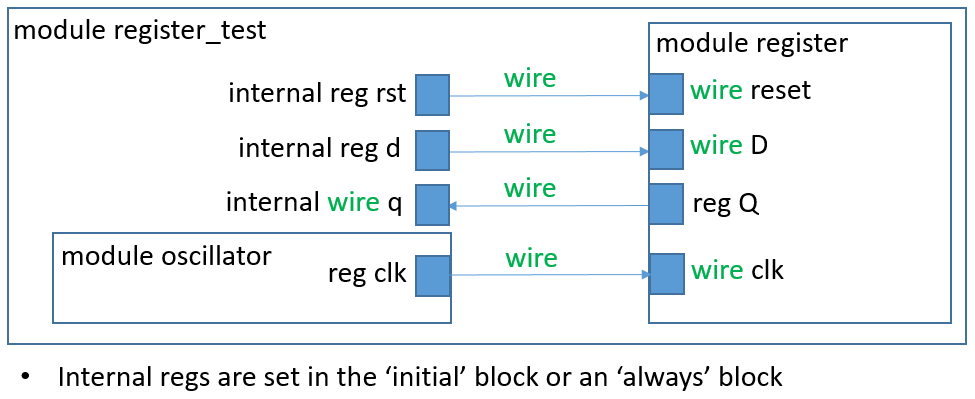
\includegraphics[width=4.75in]{../images/register_test_module_diagram.png}
	\end{center}
\end{figure}

If you don't specify anything for the port type, you will get a wire - it is the default.  In our case we have four signals: three inputs, and one output that is a register.  The first two inputs are single-bit wires.  One is the clock, which specifies the timing, and the other is reset, which clears the contents of the register (makes them zero).  The final input is the value we want to store in memory, and I have called it D, following the convention of digital logic.  D has multiple bits that are numbered from WORD-1 down to 0.  Thus the leftmost bit is 63 in this case, and the rightmost bit is 0\footnote{If you want to be technical this is called little endian, since the little end (the least significant or unit bit) is going into the first memory location (bit 0).  If you reversed the order by putting the 0 first and the WORD-1 last it would be big endian, since the big end (most significant bit) would go in the lowest addressed bit.}.  The output Q (also the digital logic conventional name) is a register (it will hold its value) and should also be of size WORD and follow the same order as the input D.

To help clarify this, please examine Figure~\ref{fig:modulediagram}, which shows the interconnection of the modules in this lab.

The final section is the body or implementation.  It is composed of a single thread of code, that will keep running (hence always).  It will run one time every time there is a positive edge (0 to 1 transition) for either the clock or reset.  Reset has higher priority, so if reset is asserted the register is cleared (Q is set to zero), otherwise the value of D is stored it Q.  That is it.  A nice, simple module.

\section{Testbench}

We now want to test this.  To test it, we need to tell the simulator to build a copy (instantiate) the module, and then we will need to supply the inputs and look at the outputs to verify that the module works correctly.  Consider the testbench in Listing~\ref{code:register_test}.

\Verilog{Verilog code to test a register.}{code:register_test}{../code/1_fetch/register_test.v}

Like our register it starts with our standard header, but this time there are no ports!  A testbench is providing all the signals to simulate the inputs to the unit under test (UUT) and thus does not need them.  This is how Verilog finds a top level simulation module - there are no ports.  The clock signal will be driven by a module named oscillator, which will give us a nice square wave with period CYCLE, which is another constant defined in our definitions.vh file.  The code thus makes an oscillator and a register, then runs the 'initial' section (it runs once at the start then never again).  The initial section sets the value of the inputs then waits a CYCLE.  The last couple of delays are not full cycles.  I did this for two reasons:
\begin{enumerate}
\item To show you how to make Verilog do calculations for you.
\item To remind you that the input won't necessarily be nice and perfectly timed to your register.  Unsynchronized signals happen, and is a frequent cause of problems, hence the need to test.
\end{enumerate}
This is by no means an exhaustive testbench, but run it and look at the output.  Does it do what you expect?  What else might you want to test?  Add this to your testbench and run it again to see if the register works.



\begin{figure}
\caption{Timing diagram.}\label{fig:registertiming}
\begin{center}
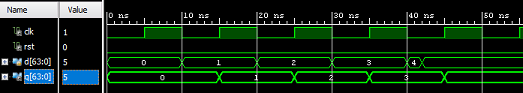
\includegraphics[width=4.75in]{../images/register_test_timing_diagram.png}
\end{center}
\end{figure}

\section{Using \LaTeX\ for Your Write-up}
This section was originally written by Dr. Schubert, so any first person references are from Dr. Schubert.

All that is left is to write it up.  I am going to have you use \LaTeX\ to do your lab reports. Note how I include files, programs, and images.  It is worth noting that \LaTeX\ will automatically make the table of contents and bibliography for you also.

Why use \LaTeX\ ?  There are lots of reasons, but here are a few that matter in this course:
\begin{enumerate}
\item It typesets programs from the actual source, no need to copy the program and have spell checkers and grammar editors mess things up.
\item It quickly and correctly handles equations.
\item It automatically handles table of contents and bibliographies.
\item It is free, and generates high quality documents (book quality) - it is open source since before open source.
\item It is used in publication of research documents.
\item It is the only large program believed to be error free in its source code, and have no missing features (development is complete!)
\end{enumerate}


\subsection{Background}

\TeX\ refers to both a language for typesetting and the program (compiler actually) that does the typesetting.  \LaTeX\ is a macro package which sits on top of \TeX\ and provides additional functionality, and has become synonymous with the language variant (dialect) of \TeX\ which it created.  Since \LaTeX\ is hugely popular and really useful, \TeX\ and \LaTeX\ have become synonymous to most people, and I will treat it so from now on.  A note on pronunciation: \TeX\ is in Greek letters - tau epsilon chi and hence is pronounced `tek' not tex (similar for \LaTeX\, which is pronounced `lay-tek' not latex).

\TeX\ is not a WYSIWYG (what you see is what you get) typesetting program like many editors you are familiar with, as it was designed to be a tagged language like the more recent html (yes, \TeX is older).  The idea is not to spend time thinking about how it should look, but rather to classify what it is and let the automated standards set the text by what the text is\footnote{For instance, note the chapter, section, and subsection commands in the tex files.  \LaTeX\ assigns a number, records it, the title, and page so it can automatically put it in the table of contents for you.}.  To provide flexibility and extension (and it was designed by one of the greatest computer scientists, Donald Knuth) it was set up as a programming language with a compiler.  Since \LaTeX\ is a programming language, we have a comment character \% that I had to escape by putting a \textbackslash before it to make it print.  Whitespace past the first space (word separation) is ignored, except for a blank line, which means start a new paragraph.  More than one blank line is ignored.  To get more space, you issue a command, such as \verb1\vspace{.25in}1, which puts a quarter inch of vertical space.  \LaTeX\ also knows pt (points), px (pixels), pc (pica), mm (millimeters), cm (centimeters), em (width of an `m'), and many more.  By default the space is not placed if it does not separate some object (i.e. at the top of a page), but you can force it by using \verb1\vspace*{.25in}1.  Starred commands are just versions of the main command.

There are many more commands than we could describe in this brief intro, including commands to let you define new commands and environments.  We will not need too many fancy commands, we only need to describe the commands to include figures, code, and equations.  If you want to learn more, then I have links to free manuals online at r2labs.org.

\subsection{Compile Process}

One thing that will help you a lot in working with \LaTeX\ is how the compile process works.  \TeX\ is a two pass compiler, but it does only one pass each time it runs.  Allow me a brief introduction to compilers, which is a great course if you can take it.

When you are compiling a file you have control statements (branches, loops, conditional execution statements like if or switch/case) that require you to know how many program lines ahead or behind something is in the assembled code, which you will not know at the start.   While you are often just putting in a flag or label to be handled by the assembler later, you in truth don't even know if they actually put the destination of the transfer of control, and thus have an error.  One easy way of handling this is to run through the process twice, collecting labels and such the first time and then doing the compile the second time through, which is what a two pass compiler does.  \TeX\ collects all the labels, notes all the chapter, section, and other structures, identifies all the bibliography references, and so on and puts them in a special auxiliary file for the next pass.  It will also create a DVI file, which has most things right, but will lack table of contents, references, bibliography, and such.  The second time through it already has the information before the file runs so it reads that first and uses it to create a fully correct output.

A logical question at this point is why not just have it run twice on its own?  Well, in the 1980's computers were small and slow, so each run of \TeX (we didn't even have \LaTeX\ at first) took an appreciable amount of time.  If you know the compile process, there are times you only have to run things once, like small spelling changes not in a title, chapter, etc.  Allowing people to do only one pass at a time was a big advantage (some \TeX\ compiles I had to do could take 10 minutes even in the 1990's).  Bibliographies are handled by an external program called BibTeX, which reads the .aux file to find the references (thus you need to run \LaTeX\ first), then pulls the data from the .bib files you specify in the calling command in your .tex file and creates a .bbl file.  The .bbl file contains all the info formatted how the bibliography should look.  \LaTeX\ reads this in the first pass and copies it over to the .aux file and resolves the links to the text references.  The next run of \LaTeX reads all this in and places both the bibliography and the cross references.  This means that to get a bibliography in you must run \LaTeX\, BibTeX, \LaTeX\, then \LaTeX\ once more.  You only need to do this if you add new reference, which in the labs will be once, provided you don't delete those intermediary files.

\subsection{Getting Started with LaTex}

Now that you have some background knowledge, we need to learn how to build a document on your computer.  There are many ways to do this, including text editors and command line tools.  I prefer using a more user-friendly editing and buidling environment.  While there are numerous options available, I choose to use TexStudio.  It is installed on all ECS computers, and it is available for free download at home.  I would recommend opening LabN.tex and building it before making any changes.  Then make some changes, rebuild, and view those changes in the PDF that is generated.  Steps to build a document in TexStudio are:
\begin{enumerate}
	\item Open TexStudio on your lab computer
	\item Use the menus open LabN.tex
	\item Click on the double green arrow icon near the top.  If you hover over it, it says "Build \& View".
	\item This should produce a PDF document on the right side of the TexStudio window
\end{enumerate}

This document should build properly as long as you don't modify it.  Once you start editing, it is possible that you will get compile errors.  These errors are listed in the bottom pane of TexStudio.  Like many compilers, they are sometimes cryptic and don't lead you directly to the problem.  The most common problem (by far) is using an underscore with using the escape character (backslash) first.  For example, look at the fetch1.tex file to see how I made this  example\_of\_how\_to\_use\_underscores.

Note that all code and image references are relative to where the .tex document is located in the file system.  It is important that you maintain the same file structure that I gave you so that these references are simple and consistent.

\section{Your Assignment}

You are to:
\begin{enumerate}
\item Finish the testbench in Listing~\ref{code:register_test} by testing several additional cases.  For instance, what happens when D is set at different points during the clock cycle, or if D is set for longer than a single clock cycle.  Also, reset is not currently being tested.  Does reset work properly?  Does the register work properly after reset has been cleared?
\item Run a simulation and generate a timing diagram.
\item Write up a lab report in \LaTeX\ following the lab format in \verb1LabN.tex1 and generate a pdf file.
\item Upload the pdf and all the Verilog files to Canvas.
\end{enumerate} 

\chapter{Program Counter Incrementer and Mux}

As mentioned in the last lab, the program counter is a register that is one word in length.  It holds the address in memory of the next instruction to be fetched and executed.  There are several ways that the program counter is updated:  
\begin{enumerate}
	\item If the program does not branch (via an if statement, while loop, etc), then the program counter should advance to the next address (by adding 4 to the current PC) each clock cycle.
	\item If the conditions of a conditional branch are met, then the program counter should be updated with the branch destination address.
	\item If an unconditional branch or jump occurs, then the program counter should be updated with the branch destination address.
	\item If an interrupt or error occurs, then the program counter should be updated with the interrupt or error handler address.
\end{enumerate}
The instructions will be fetched in sequential order the majority of the time.

\section{Incrementer}

We will build a program counter incrementer by making a simple adder.  Later in our computer we will need another adder, so we will re-use this code.  When used as the program counter, we will pass it a 4 because each instruction is 32-bits long (even though it is a 64-bit computer) and we want to increment to the next instruction in memory.  Most machines are byte addressable, because one ASCII character (a char in c/c++) is a byte.  For a machine with 32-bit instructions like we are using, that would mean that each instruction would be 4 bytes later in memory ($32/8=4$ bytes).  Therefore, we will be adding 4 to the program counter each time we want to increment the program counter.

An adder is very simple in Verilog.  There are two inputs (the two numbers to be added) and one output (the result).   All the ports are size word because they hold integers.  

In this lab you will make your own adder module.  Your adder module should be called 'adder' and should have inputs of \verb1a_in1 and \verb1b_in1.  The output should be \verb1add_out1.  HINT: this should be very easy.  Verilog is a Hardware Description Language, so use Verilog to describe what you want to do.  Don't make it complicated.  The adder code should be stored in ARM-Lab/code/0\_common/adder.v.  You will need to create this file.

\section{Input Selection via Mux}

We will also need to be able to choose between normal advancing (sequential stepping) and branching (loops, if statements, etc.).  We will use a multiplexor (mux) to do this.  A mux is a simple device that connects one of the inputs to the output based on how the control bit is set.  If the control bit is 0 then input a is connected to the output, and if the selector is 1 then input b is connected to the output.  One interesting addition in this block of code is the addition of a size parameter.  Parameters are passed before the normal ports and are used to configure the code to meet a requirement at the time of construction.  Note parameters are constants and cannot be changed later in the module.  The $=8$ defines the default value if nothing is specified.  In this case we are using parameters to set the number of wires that compose the inputs and output.  In our lab project, we will need some muxes to switch entire words (64 bits), but later we will also need to switch register addresses (5 bits).  Rather than write two muxes, we will make one and then use the parameter to change the size when they are declared.  The mux code should be stored in ARM-Lab/code/0\_common/mux.v.  Please look at the starter code in this lab document for direction on how to add a parameter to the module.

\Verilog{Verilog code to make a mux.}{code:mux}{../code/0_common/mux.v}

Look at the testbench provided for the mux.  Note that if the parameter is not set by the testbench, the mux module will set the inputs and outputs to be the default of 8.  We are going to change this to test it as a 64 bit mux and a 5-bit mux.  Notice how the size of the mux is set, since you will need to do this in future labs.

\section{Your Assignment}

You are to:
\begin{enumerate}
\item Create an adder module.
\item Use the provided adder\_test.sv to verify that the adder works properly.  Note that you cannot/should not make any changes to the test bench.  The correct results are already in the test bench.	
\item Create a mux module.
\item Use the provided mux\_test.sv to verify that the mux works properly.  Note that you cannot/should not make any changes to the test bench.  The correct results are already in the test bench.	
\item Rather than writing a lab report, please produce a landscape mode single page PDF called Lab2\_lastname.pdf that includes (in this order):
\begin{enumerate}
	\item Your name and the lab number.
	\item A snip of the Simulation Results for the adder.  Make sure to show all values in decimal form and don't cut off the signal names on the left.  
	\item A snip of the test results from the Tcl Console for the adder.  This snip should show the entire log from BEGIN TEST RESULTS to END TEST RESULTS.
	\item A snip of the Simulation Results for the mux.  Make sure to show all values in decimal form and don't cut off the signal names on the left.  
	\item A snip of the test results from the Tcl Console for the mux.  This snip should show the entire log from BEGIN TEST RESULTS to END TEST RESULTS.	
\end{enumerate}
\item Upload Lab2\_lastname.pdf file to Canvas.
\item Zip up your ARM-Lab directory and submit it on Canvas as well.  I will run your code against my correct testbench to verify that your code and testbench work correctly. 
\end{enumerate} 
\chapter{Fetch Stage}

We are ready to build our fetch stage.  To do this, we will make one more module, our instruction memory.  Then we will make a module to assemble all of our modules together into a working fetch stage.


\section{Instruction Memory Module}
Instructions are stored in memory and are accessed by using the address where they are stored.  You can think of memory like a giant hotel for our data.  Each piece of data is stored in a room (memory location), which we can find by its room number (memory address).  To get a piece of data stored in memory (like an instruction) we need to take its address, go to that location, and grab the data.  In Verilog, a bunch of memory locations that are accessed by an address is called an array.  Arrays in Verilog are declared like they are in C; the data type is specified, then the name, then the array size.  

To store the instructions, we will need an array of 32-bit numbers (definitions.vh defines INSTR\_LEN as 32, please use this macro), which means the data type must be \verb2reg[`INSTR_LEN-1:0]2.  After the name is specified (imem in this case), we are going to use a parameter called SIZE to specify how many elements the array has: \verb2[SIZE-1:0]2.  Therefore, your array will be defined as \verb2reg[`INSTR_LEN-1:0] imem [SIZE-1:0]2.

Now we need to populate this array with instructions.  Rather than populating the array element by element, we will read the instruction values in from a file called instrData.data that I have provided in the testfiles area of the ARM-Lab repository.  Note that we are just initializing the array with the values from the file.  The values should only be read from the file once at the beginning of the simulation.  Then we will access the imem array for an instruction value. To read the file and put the contents into our imem array, we will use \$readmemh to read in hexadecimal values from instrData.data.  \$readmemb could be used if we chose to format our data file in binary rather than hexadecimal.  It is very important that we use a macro in definitions.vh for the name and path of the instrData.data file, as this might change and it will be necessary for grading.  Make sure to update the definition of IMEMFILE to point to your ARM-Lab/testfiles directory (as opposed to the potter/ARM-Lab/testfiles directory).  The line of code to read the data in from the file is \verb2$readmemh(`IMEMFILE, imem);2

Once the array is populated, we can access imem and provide the instruction that corresponds to the requested address.  Instructions should only be updated on the positive edge of the clock.  I have provided a complete testbench for this module.  I have also provided a partially complete file called instr\_mem.v in code/1\_fetch directory.  Complete the module code to make a working instruction memory module.  Test it against instr\_mem\_test.sv and verify that the module works as expected.  The test will compare your instruction output to the instruction values that I provided in instrData.data. 

\section{Fetch Stage}
Now we need to connect our modules together to make a fetch stage.  The components of our instruction fetch (sometimes called ifetch or just fetch) stage are shown in Figure~\ref{fig:fetch}.

\begin{wrapfigure}{L}{2in}
\caption{Instruction Fetch Stage.}\label{fig:fetch}
\begin{center}
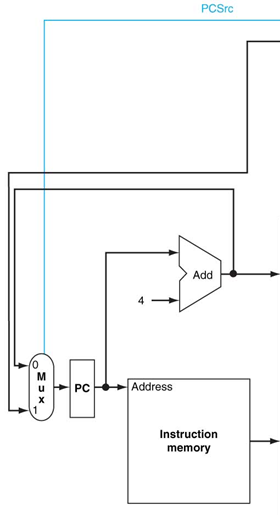
\includegraphics[width=2in]{../images/pipeline_fetch.png}
\end{center}
\end{wrapfigure}

Any wire (or reg) that comes into or goes out of the figure are input or output ports of the iFetch module.  In Figure~\ref{fig:fetch}, the blue wire is a control signal and comes ultimately from the control unit, which you will build in the decode stage.   Wires (or regs) that are completely contained in the figure are local to the iFetch module and are thus defined internally in the module (not an input or output).  The one exception to this is the current program counter (cur\_pc).  While there is no reason (at this point) that it must be output from the iFetch module, you must still make it an output so that it shows up on your simulation results, helping you to keep track of the program counter for the instruction that is currently executing.  And it is required to verify functionality with the testbench.

While the input and output signals are easily identified by the diagram, you must also determine the size of each signal and whether it is a wire or reg.  When you look at the figure I cut from a figure in the book, note that I labeled every wire on the diagram in green.  For the sake of consistency and debugging, it is required that you use these names.  

IMPORTANT NOTE: Throughout your entire project, your signal names should follow the convention of the Freescale Semiconductor Verilog guide, which states that signal names should be all lower case, with words separated by an underscore.   

Once you have figured out all your connecting signals (wires and regs), you should identify the components you are going to use.  We have already created the modules, so now we just need to tell Verilog to instantiate them in the iFetch module and connect them together.  Create the iFetch module in a new file called iFetch.v in the code/1\_fetch directory.  

I have provided a complete testbench called iFetch\_test.sv.  Use this testbench to determine if your fetch stage is working properly.  As we progress through this lab project, you will learn how critical timing is.  Please look at the cur\_pc value and the instruction value and verify that the instruction that was fetched is the correct instruction, according to instrData.data and the current program counter.  Note that no instruction should be fetched in the first 5ns, as this is a half clock cycle and does not have a rising edge.  

I have included a file called delay.v in code/0\_common.  It includes a module that inputs a clock signal and outputs a clock signal that is delayed by some number of ns.  This will be useful when resolving timing issues.  Throughout this entire lab project, the delay module should only be instantiated in the top-level module (testbench).  If you need the output of the delay function in a lower-level module, add a port to the lower-level module and pass it through that port.


\section{Your Assignment}
You are to:
\begin{enumerate}
\item Complete the instruction memory module.
\item Verify the module by running against the provided testbench.
\item Create the iFetch stage.
\item Verify the module by running against the provided testbench.
\item Produce a landscape mode PDF called Lab3\_lastname.pdf that includes (in this order):
\begin{enumerate}
\item Your name and the lab number.
\item A snip of the Simulation Results for the instr\_mem\_test.  Please show all values in decimal except for the instructions.  Please show instructions in hex.
\item The instr\_mem\_test results copied and pasted from the Tcl Console.  The results should show the entire log from BEGIN TEST RESULTS to END TEST RESULTS.
\item A snip of the Simulation Results for the iFetch\_test.  Please show all values in decimal except for the instructions.  Please show instructions in hex.  
\item The iFetch\_test results copied and pasted from the Tcl Console.  The results should show the entire log from BEGIN TEST RESULTS to END TEST RESULTS.
\end{enumerate}
\item Upload Lab3\_lastname.pdf file to Canvas.
\item Zip up your ARM-Lab directory and submit it on Canvas as well.  Please make sure that you give me the ARM-Lab directory rather than the ARM-Project directory.  I do not want the project files in the ARM-Project directory.  Before you submit your zip file, extract the file and make sure that the top-level directory is called ARM-Lab and that the lower level directories like code, manual, etc are directly beneath ARM-Lab in the directory structure.  I will extract your zip file and run your code against my correct testbench to verify that your code and testbench work correctly, and it is critical that everyone's directory structure is consistent.
\end{enumerate} 
\chapter{Beginning to Decode}

\section{Instruction Decode}

The next stage in the datapath is the iDecode stage.  The iDecode stage evaluates the binary instructions (an output of the iFetch stage) and determines what needs to be done.  There are many aspects to the iDecode stage, and some get fairly complex.  But today we will begin the process of decoding an instruction by decomposing the instructions into the key parts of R-Type and D-Type instructions:
\begin{enumerate}
	\item opcode
	\item address (used only in D-Type instructions)
	\item rm\_num (used only in R-Type instructions)
	\item rn\_num
	\item rd\_num (though the book uses Rt for D-type instructions, we will use Rd for the last operand of D-type instructions)
\end{enumerate}   

To do this, you will create a new module called instr\_parse.  This module will simply read inputs and assign appropriate output values.  These outputs should be assigned using continuous assignments.  The input is a 32-bit instruction.  Outputs are listed for you above.  Although R-type and D-type instructions have different operands, you can treat them the same for now.  For instance, you can still assign an Address field on an R-type instruction, and you can still assign an Rm field on a D-type instruction.  When we create the Control Module in a future lab, the control signals will drive what fields of the instruction are used and what fields are ignored.  Notice how, because of the commonality of instruction format, Opcode, Rn, and Rd are all universal across these instruction types.  Please remember to use the style specified in the previous lab, where all items are lower case with underscores separating them.  For instance, for Rd, you should use the signal name rd\_num.  Appending num on the end of the name indicates that this is the register number, not the value from the register.

To test this module, you will need to create an instr\_parse\_test.v that will feed the module with instructions.  Since we are not integrating with our fetch module yet, your test bench should manually set the instruction values.  I am providing the testbench, shown in Listing~\ref{code:instr_parse_test}..  For instruction inputs, it uses three of the four instructions that we recently decomposed in the lecture on machine code.  I modified the ADD instruction slightly to use X10 as the destination register.  I do not include the ADDI instruction because we will not be implementing immediate instructions in lab.  Please make an Expected Results Table and use it to verify that your instructions are being parsed correctly.

\Verilog{Instruction Parse Testbench}{code:instr_parse_test}{../code/2_Decode/instr_parse_test.v}

\section{Register File}

Next, we will create the register file.  The register file is a piece of memory in the processor that holds the 32 register values that are used by most instructions (X0-X31).  You will create a new module called regfile (in regfile.v).  The regfile module should retrieve data from the registers on the rising edge of read\_clk as well as write to the registers on the rising edge of write\_clk when the regWrite flag is set.  Two different clocks are used here because the regfile will be read at a different time than it is written to.  The regfile should use a verilog reg array.  You should not use the register module that you used for your program counter.  Since we don't currently have the ability to do loads and stores (since we don't have data memory yet), the values for the registers should be stored in a datafile, regData.data and copied into the array during the initial block, just like we did with the instr\_mem.v file.  regData.data is provided for you.  The regfile module will have a lot of similarities to the instr\_mem module, so I recommend reusing concepts and code from the instr\_mem module.

Inputs to the module should include a signal called read\_clk and a signal called write\_clk as well as all inputs shown on the Register file in Figure~\ref{fig:register_file_cutout}.  Don't forget reg\_write.  This is a control signal that determines whether data should be written to the register.  Some instruction write to registers, others do not.  The outputs should be the outputs of the Register file in Figure~\ref{fig:register_file_cutout}.  Use names such as read\_register1, read\_data2, etc.

You will need to write a testbench, regfile\_test.v, for this module as well.  It should provide values for each input and verify that the outputs match expected behavior.  You should use the delay module in your testbench to create different clocks for read\_clk and write\_clk.  Recommended test cases include:

\begin{enumerate}
	\item Set Read Register 1 and verify that Read Data 1 contains the correct data, according the regData.data.  Repeat this for several different Read Register 1 values.
	\item Set Read Register 2 and verify that Read Data 2 contains the correct data, according the regData.data.  Repeat this for several different Read Register 2 values.
	\item Write data to the Write Register, then set Read Register 1 to that register and verify that the value has been updated to the value that you wrote to Write Register.
	\item Change Write Register, then write data to the Write Register, then set Read Register 2 to that register and verify that the value has been updated to the value that you wrote to Write Register.
	\item Repeat the last 2 steps but have reg\_write set to 0 and verify that the register value does not get updated.
\end{enumerate} 

\begin{figure}
	\caption{Expected Results}\label{fig:register_file_cutout}
	\begin{center}
		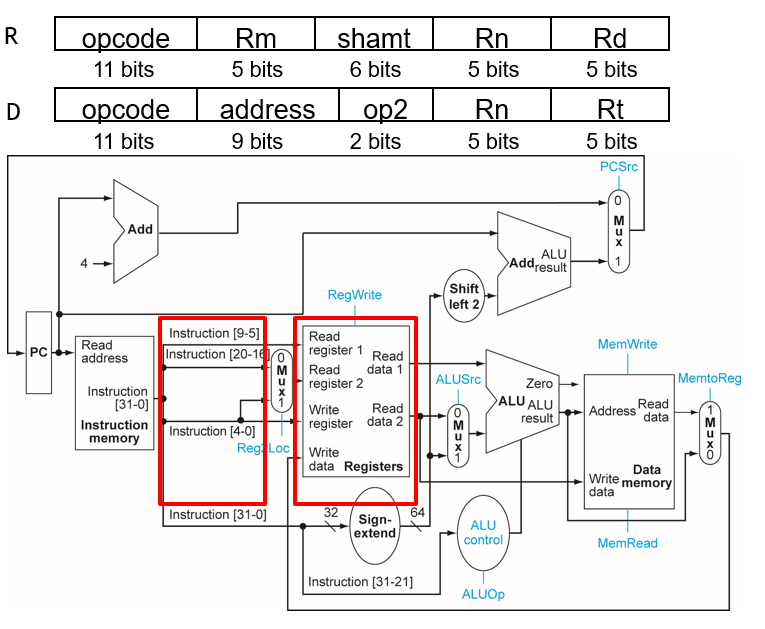
\includegraphics[width=4.75in]{../images/register_file_cutout.png}
	\end{center}
\end{figure} 


\clearpage
\section{Your Assignment}

You are to:
\begin{enumerate}
\item Create an instr\_parse module as described above.
\item Create and Expected Results Table for instr\_parse\_test.
\item Use the instr\_parse test module and verify that the instruction is being parsed properly by comparing to the Expected Results Table.
\item Create a regfile module.
\item Create a regfile\_test module.
\item Create an Expected Results Table for regfile\_test.
\item Verify that the values are being stored and retrieved from the regfile properly by comparing the results with the Expected Results Table.
\item Write a lab report according to the LabN format.
\end{enumerate} 
\chapter{Register File}

\section{Register File}

Next, we will create the register file.  You will create a new module called regfile (in regfile.v), and this module will be part of your iDecode module.  The regfile module should retrieve data from the registers as well as write to the registers when the regWrite flag is set and the clock edge rises.  The regfile should use a verilog reg array.  You do not need to use the register module that you used for your program counter.  Since we don't currently have the ability to do loads and stores (since we don't have data memory yet), the values for the registers should be stored in a datafile, fibR.data and read in during the initial block.  In order to get results that match my provided results (and match the provided unit test), you should set X21=16, X9=33, X10=12 in fibR.data.

A unit test is provided, iDecode\_test.v.  It simply sends two commands (the add and subtract commands from last lab) and sets a few flags.  Using that unit test, you should be able to produce the results shown in the lab manual.  Note that in addition to the register file, you will also need to create a mux to determine the source of the second read register.  Note that because we are sending the instructions from the test instead of from the iFetch routine, you will need to update your code from last lab to use procedural statements triggered on the clock edge.  Otherwise, the instructions will not come in on the clock edge as expected.  Timing is very important in this lab.

\begin{figure}
	\caption{Expected Results}\label{fig:register_file_cutout}
	\begin{center}
		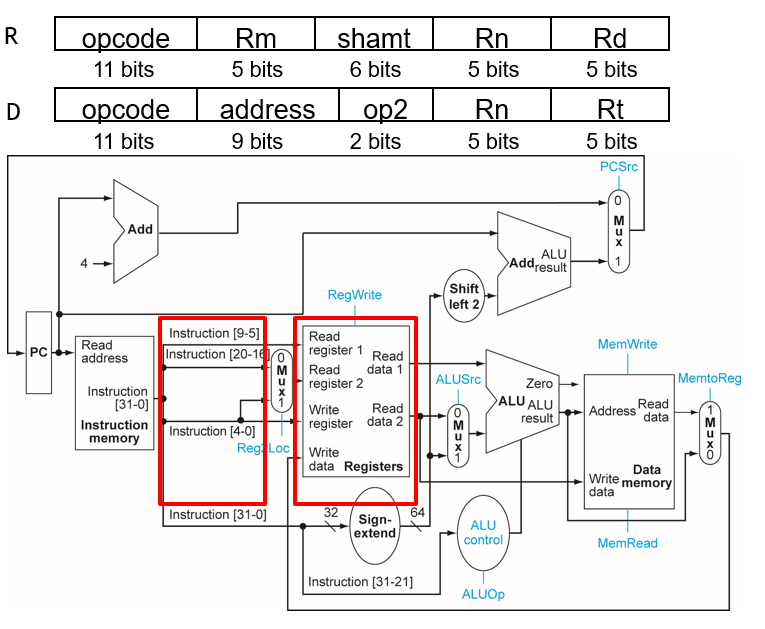
\includegraphics[width=4.75in]{../images/register_file_cutout.png}
	\end{center}
\end{figure} 

\Verilog{Verilog starter code for the iDecode module.}{code:iDecode_reg_test_version}{../code/2_decode/iDecode_reg_test_version.v}

\begin{figure}
	\caption{Expected Results}\label{fig:register_file_test_output}
	\begin{center}
		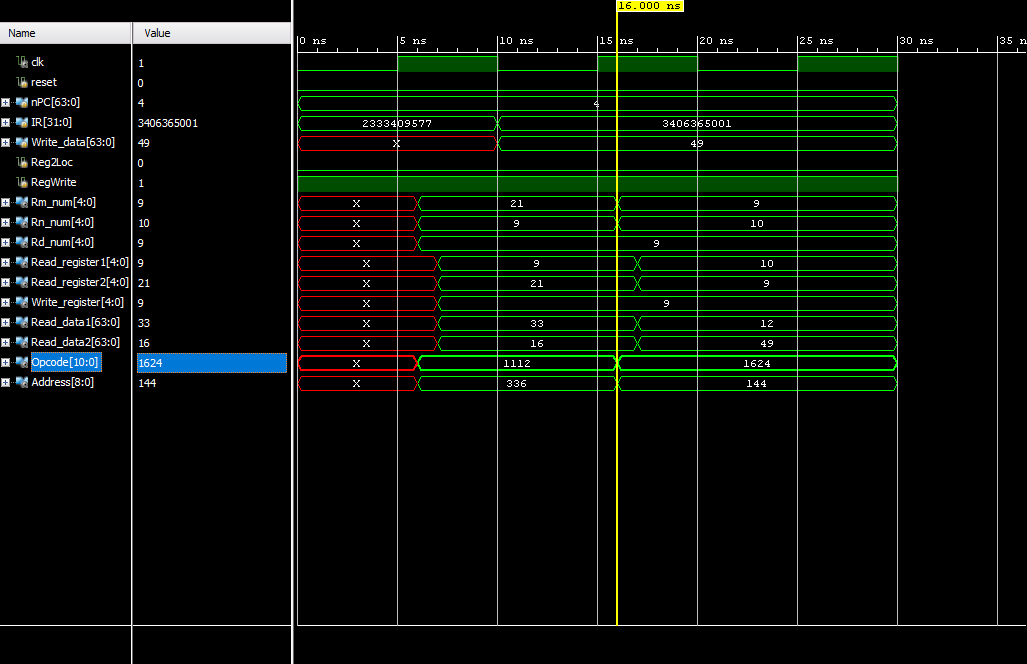
\includegraphics[width=6.75in]{../images/register_file_test_output.png}
	\end{center}
\end{figure}

\clearpage
\section{Your Assignment}

You are to:
\begin{enumerate}
\item Create a regfile module and add it to the iDecode module.
\item Re-use your mux from previous labs and add it to the iDecode module.
\item Import the provided iDecode\_test.v file.
\item Verify that your results match the expected results.
\item There will not be a submittal on Canvas today.  However, please show me your results either today or at the beginning of lab time during the next class period.  We will be adding more functionality next time.
\end{enumerate} 
\chapter{Finishing Decode}

\section{iDecode Module}
At this point, you have created all of the modules necessary to assemble the iDecode module.  Now you need to create a new module called iDecode.  The inputs and outputs can be determined by evaluating Figure~\ref{fig:decode_stage}.  Any signal that crosses the boundaries of the red box is an input or output.  Signals that do not cross the boundaries of the red box are signals that are internal to the iDecode module and should be declared internally in iDecode.  Please make sure to label signals consistently with lower case letters with words separated by underscores.  For example, read\_data1, write\_data, alu\_src.

\begin{figure}
	\caption{Expected Results}\label{fig:decode_stage}
	\begin{center}
		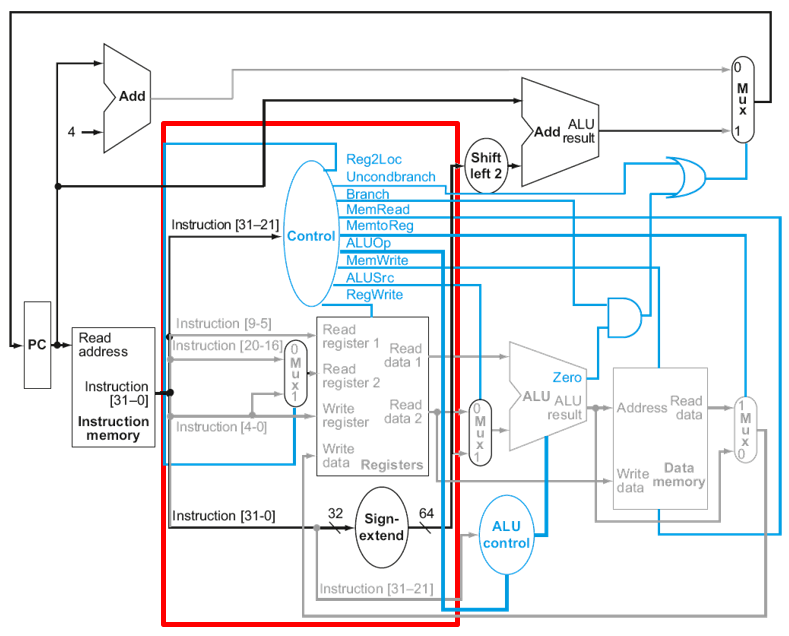
\includegraphics[width=4.75in]{../images/decode_stage.png}
	\end{center}
\end{figure} 


\section{iDecode Unit Test}
To verify that your iDecode module works correctly, you must first update your Expected Results Table. You should first add a row for every input and output of your iDecode module, then fill in all cells with expected values.  If a particular data item is not relevant for a particular instruction (for instance, sign\_extended\_output on an R-type instruction), then just put an X in that cell.  To ensure that we are testing each case, please update regData.data to reflect the following values:

\begin{enumerate}
	\item X19 = 10
	\item X20 = 30
	\item X21 = 0
	\item X22 = 16
\end{enumerate}

Now create a unit test for iDecode by providing the inputs for iDecode and verifying the outputs of iDecode.  For the instruction input, use the instructions from your Expected Results Table.  For arithmetic instructions, use the test bench to provide the correct value to the write\_data input, since we do not yet have an ALU to do the calculations.  Also, please use your test bench to provide a value of 20 to X9 in the first command (LDUR).

With your Expected Results Table in hand, you should be able to run the iDecode unit test and analyze your simulation outputs by going vertically down the simulation output, comparing the table to your simulation output.  While certain values will be offset in time, a single instruction should fall within a single clock cycle.  

\section{Integrating iFetch and iDecode}
Now that you have iDecode created and tested, you can test it with your iFetch module.  To do this, you need to create a file called datapath.v.  This will be your top-level file for your integrated datapath, analagous to the test bench files.  In this file, you should have an instance of iFetch and iDecode.  You should connect these two modules with wires by analyzing the full datapath diagram.  Since we do not have a full datapath yet, we need to have some "test bench" aspects to datapath.v.  Similarly to your iFetch test, you will want to create a reg for reset, pc\_src, and branch\_target.  Since we do not have all aspects of branching implemented, please keep pc\_src set to 0 for the duration of the test.  

Please update your instrData.data file to only contain the 10 instructions in your Expected Results Table.  The goal of datapath.v is to verify that the PC increments, each of these instructions is fetched at the appropriate time, and that the instruction executes properly.  You can verify the execution by comparing your results with your expected results table.     

\section{Your Assignment}

You are to:
\begin{enumerate}
\item Integrate all individual modules into the iDecode module.
\item Update your Expected Results Table to include all iDecode inputs and outputs.
\item Test the iDecode module with the instructions from the Expected Results Table.
\item Verify that your simulation results match your expected results.
\item Create datapath.v and integrate the iFetch and iDecode stages.
\item Verify that the results match the Expected Results Table.
\item Write a lab report according to the LabN format.  The focus of the report is the iDecode module, including testing it with iDecode\_test and integrating it with iFetch.  It does not need to describe the details of the submodules...you have already written a report on those.  Please consider datapath.v to be a testbench when writing the report.
\end{enumerate} 
\chapter{Integrating Fetch and Decode}

This lab will integrate the iFetch module with the iDecode module to make a single testbench that will verify that they function properly together.  The result will be a system that automatically fetches instructions and then decodes the fetched instruction.  To do this, you will update the provided fd\_integration.sv to include an instance of both the iFetch module and the iDecode module.  The instruction output from the fetch module should be connected to the instruction input in the decode module.  

You will also need to thoroughly test the outputs of each stage.  Refer back to your iFetch\_test.sv and iDecode\_test.sv files to identify what you need to test.  You will need to verify every item that you verified in each of those previous tests.  We will be using the instructions and expected values from the Expected Results Table in the iDecode lab.  Note that this time, rather than providing the instructions in the testbench, the iFetch module should provide the instructions.  This means that you will need to update instrData.data with the 10 instructions from the Expected Results Table.  Make sure to also verify the cur\_pc and instruction outputs of the iFetch module.  Overall, the tests should have 139 steps.  119 come from the iDecode signals and 20 come from the iFetch signals.


\section{Your Assignment}

You are to:
\begin{enumerate}
\item Update the provided fd\_integration.sv by instantiating iFetch and iDecode modules.  Also, update fd\_integration.sv with values from the Expected Results Table and with expected outputs from iFetch. 
\item Verify that your simulation results match your expected results.
\item Rather than writing a lab report, please produce a landscape mode PDF file called Lab7\_lastname.pdf that includes (in this order):
\begin{enumerate}
	\item Your name and the lab number.
	\item A snip of your completed Expected Results Table.
	\item A snip of the Simulation Results for the fd\_integration test.  Please show instructions in hex, opcodes and control signals in binary and everything else in signed decimal.  
	\item Copy and paste the entire log from BEGIN TEST RESULTS to END TEST RESULTS into your file.  The results have gotten too long to use the snipping tool.	
\end{enumerate}
\item Upload Lab7\_lastname.pdf file to Canvas.
\item Zip up your ARM-Lab directory and submit it on Canvas as well.  I will run your code against my correct testbench to verify that your code and testbench work correctly.
\end{enumerate} 
\chapter{ALU and ALU Control}
The goal of this lab is to build the ALU and ALU Control modules. These modules can be seen in the context of the datapath by viewing the datapath diagram from a previous lab, Figure~\ref{fig:decode_stage}.  The ALU performs the arithmetic and logical operations, and the ALU Control module determines which operation should be performed by the ALU.  During this lab, we will not put these modules together.  Instead, they will be tested independently of each other.
\section{ALU}
The ALU has three inputs:
\begin{enumerate}
	\item a\_in - the first input operand
	\item b\_in - the second input operand
	\item alu\_control - control signal used to tell the ALU what operation to perform
\end{enumerate}
The ALU has two outputs:
\begin{enumerate}
	\item alu\_result - the result of the arithmetic/logic operation
	\item zero - a flag indicating whether alu\_result is zero
\end{enumerate}  
Figure~\ref{fig:alu_control_table} identifies the operation that corresponds to the alu\_ctrl value.  Note that we will not be implementing NOR, even though it is listed in the table.  You should use a case statement to evaluate the alu\_control bits to determine which ALU operation to perform.  For each operation, you do not have to do anything fancy.  You just need to use the math capability that verilog provides to make the calculation.  To make the code readable, you must give the the ALU control bits names in the definitions.vh file, and you should use these in your cases.  Please use the following names for your macros in defintions.vh:
\begin{enumerate}
	\item ALU\_AND
	\item ALU\_ORR
	\item ALU\_ADD
	\item ALU\_SUB
	\item ALU\_PASS
\end{enumerate}
Also, don't forget to make a default case, which is needed to actually wire this up.  Please use AND for the default case.

One last thing to note is the generation of the zero flag.  The zero flag is determine by simply evaluating the alu\_result.  There are several ways to handle this, but this is the easiest way to handle it.  In Verilog (like C), the statement $(y==0)$ is an operation with a boolean output.  You can thus say $x=(y==0);$ to assign $x$ to be the boolean value that $(y==0)$ produced.  The statement $x=(y==0);$ is realizable as a digital comparator with $y$ and $0$ as inputs and $x$ as the single bit output.  Please note that you will not have signals called $x$ and $y$.  I just used these to explain the concept.

\begin{figure}
	\caption{ALU Control Values}\label{fig:alu_control_table}
	\begin{center}
		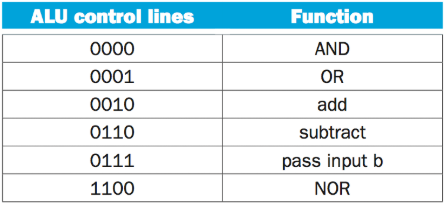
\includegraphics[width=2.75in]{../images/alu_control_table.png}
	\end{center}
\end{figure} 

\section{ALU Control}
The ALU Control module has two inputs:
\begin{enumerate}
	\item alu\_op - 2 bit signal giving incomplete information about what ALU operation should be performed
	\item opcode - the opcode of the instruction
\end{enumerate}
The ALU Control module has one output:
\begin{enumerate}
	\item alu\_control - control signal used to tell the ALU what operation to perform
\end{enumerate}
You have already defined the ALUOp macros in definitions.vh when you created the control module.  You have also already defined the ALU Control macros in definitions.vh in the previous section.  And you have macros defined for instruction opcodes. Please use these macros when creating the ALU Control module.

Figure~\ref{fig:alu_control_table} identifies the operation that corresponds to the alu\_ctrl value.  This module can be implemented multiple ways, but we want to use the most efficient way possible.  The most efficient method is to use a casex statement to evaluate the alu\_op signal, utilizing the information in Figure~\ref{fig:alu_op_opcode_table}.  alu\_op will provide all information necessary for D-Type and CB-Type instructions.  For R-Type instructions, you should use the bits of the opcode to set the alu\_ctrl value.  When evaluating Figure~\ref{fig:alu_op_opcode_table} for R-Type instructions, certain bits of the instruction correspond to alu\_ctrl bits.  The magic decoder ring is listed below.  Please note that the numbering system for the instruction bits includes the entire instruction, whereas you will just have the opcode to work with.  Therefore, you will need to adjust the numbering to account for your 11-bit opcode.
\begin{enumerate}
	\item ALU Ctrl [3] = 0
	\item ALU Ctrl [2] = I[30]
	\item ALU Ctrl [1] = I[24]
	\item ALU Ctrl [0] = I[29]
\end{enumerate} 

Please use AND as the default case.  For the B instruction, the ALU Op should be 00 from your control module.  Since 00 is also the ALU Op for LDUR and STUR (which have ALU Control value of ADD), you can just allow the B instruction to also set ALU Control to ADD.

\begin{figure}
	\caption{ALU Op Table}\label{fig:alu_op_opcode_table}
	\begin{center}
		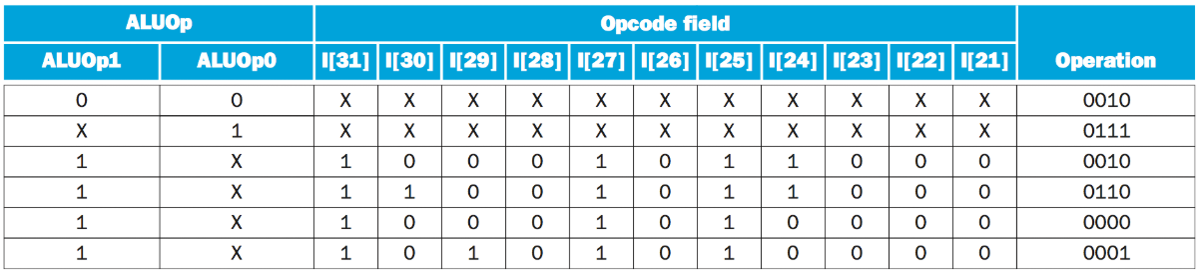
\includegraphics[width=4.75in]{../images/alu_op_opcode_table.png}
	\end{center}
\end{figure} 

\section{Your Assignment}

You are to:
\begin{enumerate}
\item Create the ALU module.
\item Verify that your ALU module works correctly by running it against the provided test bench.
\item Create an ALU Control module.
\item Verify that your ALU module works correctly by running it against the provided test bench.
\item Rather than writing a lab report, please produce a landscape mode PDF file called Lab8\_lastname.pdf that includes (in this order):
\begin{enumerate}
	\item Your name and the lab number.
	\item A snip of the Simulation Results for the each test bench.  Please show instructions in hex, opcodes and control signals in binary and everything else in signed decimal.  
	\item For each test bench, copy and paste the entire log from BEGIN TEST RESULTS to END TEST RESULTS into your file.	
\end{enumerate}
\item Upload Lab8\_lastname.pdf file to Canvas.
\item Zip up your ARM-Lab directory and submit it on Canvas as well.  I will run your code against my correct testbench to verify that your code and testbench work correctly.
\end{enumerate} 
\chapter{Execute Stage}

\section{Execute}

In the last lab, you created the ALU and ALU Control modules.  Now we will finish the iExecute stage by creating a new module called iExecute.  The iExecute module should consist of everything shown in the red box in Figure ~\ref{fig:execute_stage}.  To implement the iExecute stage, you will need to create iExecute.v and add the following components to it:
 
\begin{enumerate}
	\item ALU module from the previous lab
	\item ALU Control module from the previous lab	
	\item Mux to select the source of the second input into the ALU.  You can reuse your mux that you created in the iFetch stage.
	\item Shifter to left shift the sign extended branch address offset.  You should NOT create a new module for this.  Instead, you should add code directly in iExecute.v since the left shift can be accomplished with a single line of code. 
	\item Adder to add the branch address offset to the current PC.  You can reuse your adder that you created in the iFetch stage.  Please note the adder is near the top of the datapath diagram and it has an output named ALU result on the diagram.  In fact, this is not a full ALU, but just an adder.  And our output signal will be named branch\_target, as this is what it really is (rather than naming it ALU\_Result).
\end{enumerate} 

\begin{figure}
	\caption{Execute Stage}\label{fig:execute_stage}
	\begin{center}
		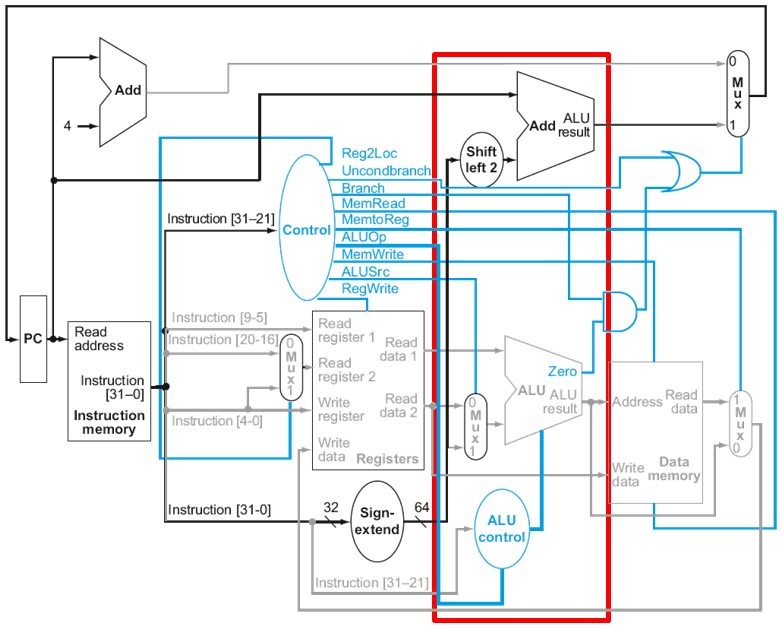
\includegraphics[width=4.75in]{../images/execute_stage.png}
	\end{center}
\end{figure} 


The testbench will run the 10 instructions in your Expected Results Table.  Therefore, your next step is to update your Expected Results Table by updating the 3 outputs of the iExecute stage. You also need to update 1 input to the table, PC.  The PC value should start at 0 and increment by 4 for each instruction.  Populate the iExecute output rows with expected values for each instruction.  All of the inputs that you need to determine the expected result are in the table.  Make sure to use N/A if the signal is not applicable for a given instruction.

Finally, you need to complete the testbench.  I have provided the bulk of the testbench.  The only updates that you need to make to the testbench are:
\begin{enumerate}
	\item I have X for all er values right now.  Please update these to the correct values per your Expected Results Table.
	\item I have a verify function call for all 3 outputs for every instruction.  If an output is N/A for a particular instruction, remove or comment out that verify.  There should be a total of 20 test cases.  
\end{enumerate}   


\section{Integrating Fetch, Decode, and Execute}
We now have working Fetch, Decode, and Execute modules.  Now it is time to put them together to produce a system that can:
\begin{enumerate}
	\item Update the program counter
	\item Read the appropriate instruction from the instruction datafile
	\item Read the correct registers
	\item Update all control lines
	\item Sign extend address data
	\item Calculate Branch Target Addresses
	\item Provide a zero bit for conditional branch instructions
	\item Produce ALU results for R-Type and D-Type instructions
\end{enumerate}

Once we can do all of this, we will be ready for the iMemory stage.  We currently have the fetch and decode module integrated into fd\_integration.sv.  We also have a working execute module.  Today we need to integrate the execute module with the fetch and decode stages.  The new testbench should be called fde\_integration.sv.  Please reuse the instructions from your Expected Results Table that you used when you integrated fetch and decode.  Once integrated, you should be able to produce a simulation that includes the outputs of fetch and decode as well as 3 new outputs from execute:
\begin{enumerate}
	\item Branch Target
	\item ALU Result
	\item Zero
\end{enumerate}   

These three new outputs are marked on Figure Figure ~\ref{fig:integrated_execute}.  To verify these outputs, you should have already  updated the Expected Results Table to include these three outputs.  To test this integration, I recommend copying the contents of fd\_integration.sv into fde\_integration.sv and then modifying from there, adding your execute module, cr values, verify statements, etc that are necessary to verify the integration of the execute module. fd\_integration had 139 test cases, so fde\_integration should have 159 test cases.

\begin{figure}
	\caption{Execute Stage}\label{fig:integrated_execute}
	\begin{center}
		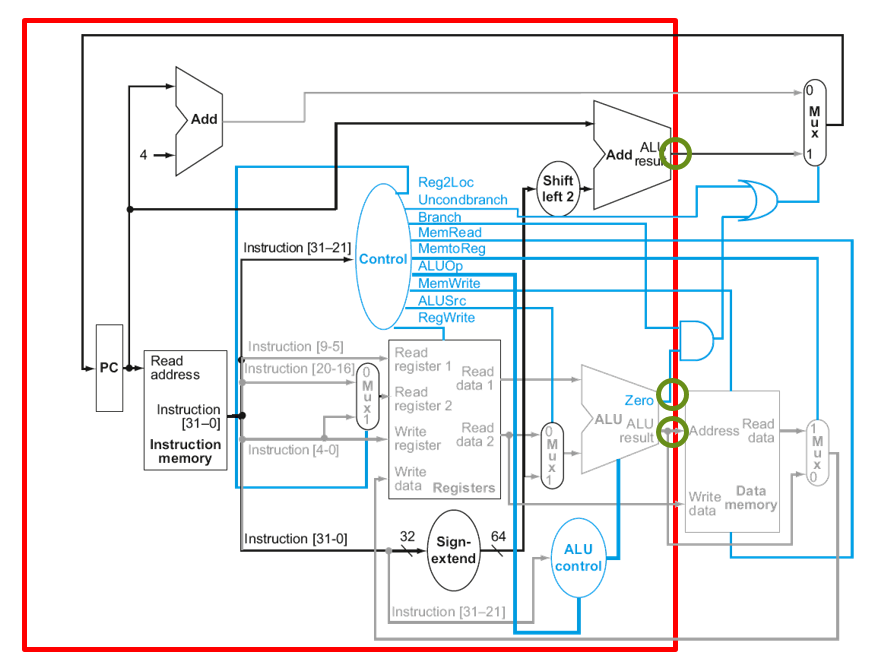
\includegraphics[width=4.75in]{../images/integrated_execute.png}
	\end{center}
\end{figure} 

\section{Your Assignment}
You are to:
\begin{enumerate}
\item Complete the iExecute module 
\item Update your Expected Results Table with the outputs from the iExecute stage.  Also add a PC value if it is not in the table yet. 
\item Update iExecute\_test.sv
\item Verify that your simulation results match your expected results.
\item Create fde\_integration.sv
\item Verify that your simulation results match your expected results.
\item Rather than writing a lab report, please produce a landscape mode PDF file called Lab9\_lastname.pdf that includes (in this order):
\begin{enumerate}
	\item Your name and the lab number.
	\item A snip of your completed Expected Results Table.
	\item A snip of the Simulation Results for the iExecute test and fde\_integration test.  Please show instructions in hex, opcodes and control signals in binary and everything else in signed decimal.  
	\item Copy and paste the entire log from BEGIN TEST RESULTS to END TEST RESULTS into your file.  The results have gotten too long to use the snipping tool.	
\end{enumerate}
\item Upload Lab9\_lastname.pdf file to Canvas.
\item Zip up your ARM-Lab directory and submit it on Canvas as well.  Please make sure that you give me the ARM-Lab directory rather than the ARM-Project directory.  I do not want the project files in the ARM-Project directory.  Before you submit your zip file, extract the file and make sure that the top-level directory is called ARM-Lab and that the lower level directories like code, manual, etc are directly beneath ARM-Lab in the directory structure.  I will extract your zip file and run your code against my correct testbench to verify that your code and testbench work correctly, and it is critical that everyone's directory structure is consistent.
\end{enumerate} 
%\chapter{Integrating Fetch and Decode}

\section{Integration}
We now have working Fetch, Decode, and Execute modules.  Now it is time to put them together to produce a system that can:
\begin{enumerate}
	\item Update the program counter
	\item Read the appropriate instruction from the instruction datafile
	\item Read the correct registers
	\item Update all control lines
	\item Sign extend address data
	\item Calculate Branch Target Addresses
	\item Provide a zero bit for conditional branch instructions
	\item Produce ALU results for R-Type and D-Type instructions
\end{enumerate}

Once we can do all of this, we will be ready for the iMemory stage.  We currently have the fetch and decode module integrated into datapath.v.  We also have a working execute module.  Today we need to integrate the Execute module into datapath.v.  Please reuse the instructions from your Expected Results Table that you used when you integrated fetch and decode.  Please make sure that datapath.v is the "top module" in your project.  Once integrated, you should be able to produce a simulation that includes 3 new outputs:
\begin{enumerate}
	\item Branch Target
	\item ALU Result
	\item Zero
\end{enumerate}   

These three new outputs are marked on Figure Figure ~\ref{fig:integrated_execute}.  To verify these outputs, you should update the Expected Results Table to include these three outputs.  Then you should verify this table against your simulation results.

\begin{figure}
	\caption{Execute Stage}\label{fig:integrated_execute}
	\begin{center}
		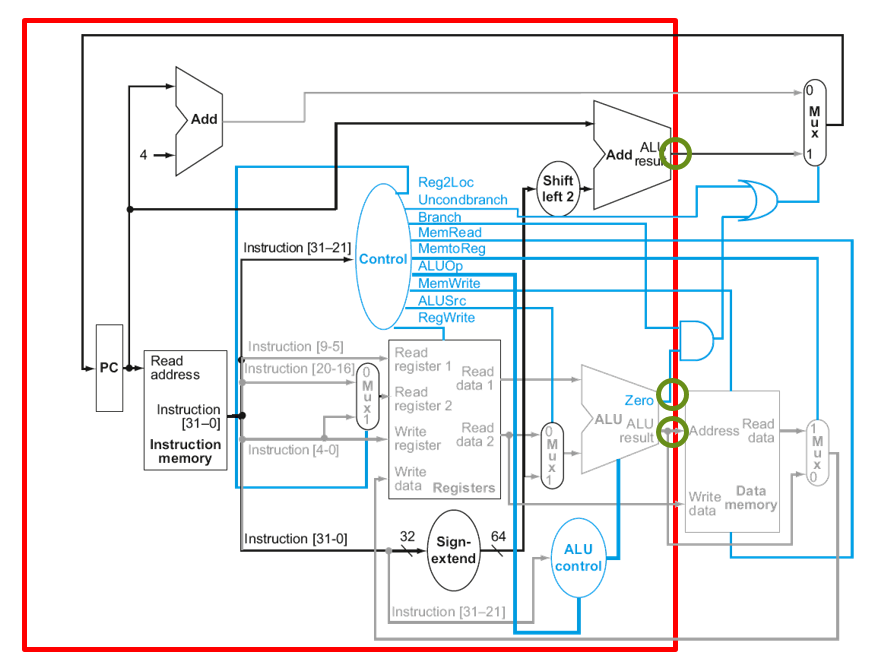
\includegraphics[width=4.75in]{../images/integrated_execute.png}
	\end{center}
\end{figure} 

\section{Your Assignment}

You are to:
\begin{enumerate}
\item Integrate your iExecute module into your datapath.v that includes iFetch and iExecute.
\item Update your Expected Results Table to include the new outputs.
\item Verify that your simulation results match your expected results.
\item Create a lab report in the LabN format that focuses on the integration of the iExecute stage.  The only inputs that you need to list are the inputs that you set in the initial section of datapath.v.  The only outputs are the signals that are leaving the red box in Figure ~\ref{fig:integrated_execute}. 
\end{enumerate}
\chapter{Memory}

\begin{center}
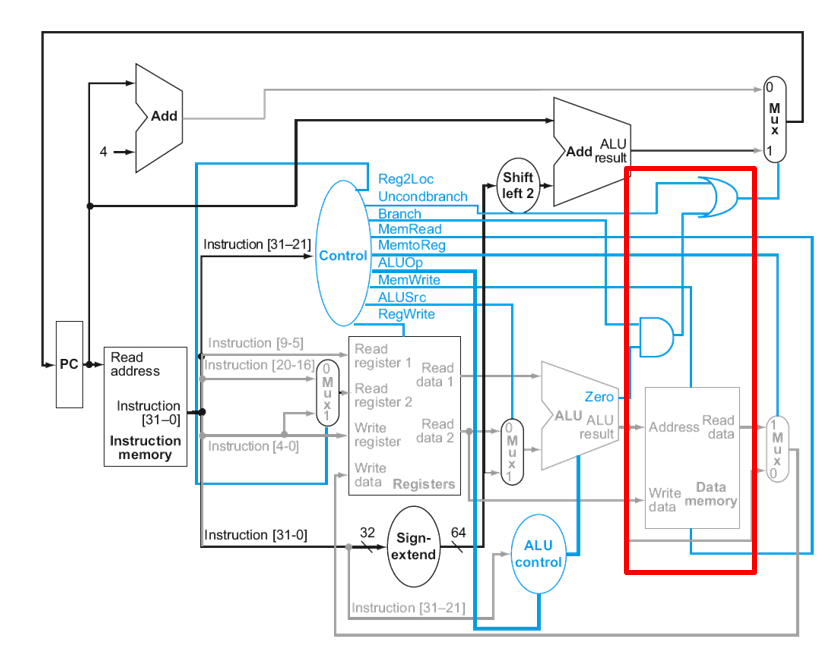
\includegraphics[width=5.5in]{../images/data_memory.png}
\end{center}

\section{Memory Stage}
Today we will create the iMemory stage of our processor.  This stage contains the data memory for the system that we use for load and store commands.  It also contains the logic gates used to produce the pc\_src signal that is used in the iFetch stage.  Note that although the diagram shows the pc\_src mux on the right side of the diagram, the mux is actually already implemented in the iFetch stage and belongs in the iFetch stage.

\section{Branch Resolution}

We now have all the information necessary to decide if the computer should branch or not.  We have the signal `branch' to tell us if it is a branch command, and we have `zero' to tell us if the condition was met.  Both branch and zero must be true so we will combine them with an `and' gate.

We also need an 'or' gate to 'or' together the output of the branch 'and' gate (above) and the uncondBranch control signal.  These gates can be included in your iMemory module as one line commands.  They do not need to be explicitly tested, as they will be thoroughly tested when we integrate the system.  

\section{Data Memory}

This will be similar to the register file memory, with two primary changes:
\begin{enumerate}
\item reading is now conditional on the MemRead control wire being high.  If the MemRead flag is not high, then the read\_data output should be set to Z (high impedance).
\item writing is now permissible if the MemWrite control wire is high.
\end{enumerate}
Create a data\_mem.v file, copy the contents of your register file memory and modify it to meet the needs of the data memory module.  You will also need to create a new data file, ramData.data that contains the initial values to be read into memory.

\section{Test Bench}
For this lab, we will just have a single test bench that will test the entire iMemory stage.  The test bench should verify the following:
\begin{enumerate}
	\item Correct logic for branching using the zero flag, branch control signal, and unconditional branch control signal
	\item That data can be read correctly from the iMemory module, verifying that you receive the correct value from ramData.data.
	\item That data can be written successfully to memory.  To verify that the write worked correctly, make sure to read from that address and verify that you read the updated value.  
\end{enumerate}


\section{Your Assignment}

You are to:
\begin{enumerate}
\item Create a new module called iMemory.
\item Instantiate the AND and OR gates directly in the iMemory stage.
\item Create a new module called data\_mem to handle data memory access.  Also create or modify a ramData.data file that contains initial values to be read into memory.
\item Integrate data\_mem into the iMemory stage.  
\item Write a testbench to verify that the iMemory stage works properly. 
\item Create a lab report in the LabN format.
\end{enumerate} 
\chapter{Write Back}


\begin{figure}
\caption{Write Back}\label{fig:wb}
\begin{center}
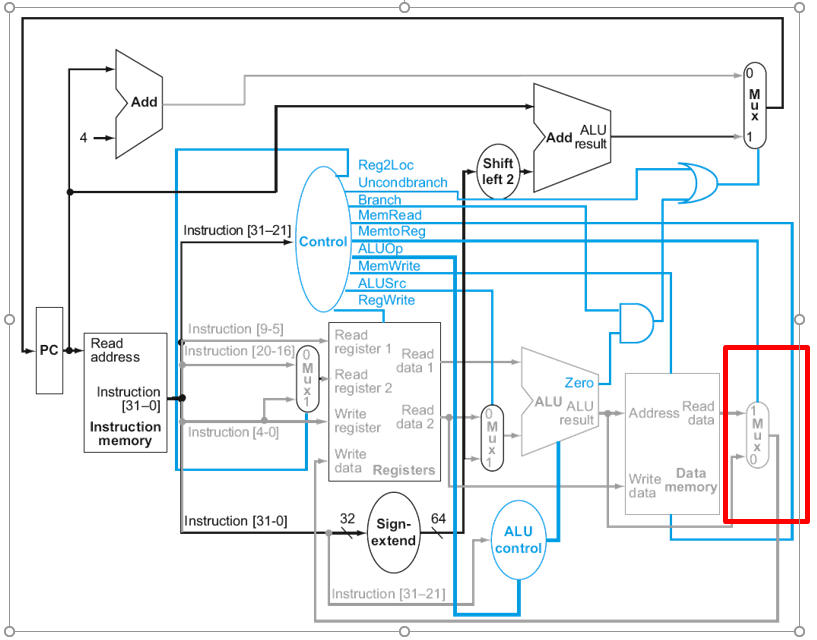
\includegraphics[width=\textwidth]{../images/writeback_stage.png}
\end{center}
\end{figure}

\WrapBarrier

\section{Mux}
This stage consists on only one item, a mux to select between the output of memory and the output of the ALU.  The control is the MemtoReg control line, see Fig~\ref{fig:wb}.  Since the mux has already been tested it does not need a testbench.  The stage thus has only 3 inputs (2 data and 1 control) and one output, the result.

\section{Datapath}
You are ready to assemble the full non-pipelined datapath shown in Fig~\ref{fig:datapath}.  To do this, you will need to combine all 5 stages into datapath.sv.  datapath.sv is a new top-level file, so it is the testbench.  Verify operation of your datapath by running your set of instructions in instrData.data and testing the output.  These instructions are the 10 instructions from the Expected Results Table.  

Now that we have a writeback stage, we do not need to set write\_data in the initial section of datapath.sv.  Rather, you should connect write\_data from the WriteBack stage to the Decode stage.  Because we now have a memory stage, we should no longer need to set pc\_src in the inital section of datapath.sv.  However, our test instructions are not meant to run like a program and would yield strange results.  So for right now, we want to keep pc\_src hard-coded to 0 in datapath.sv.  To do this, we will use a new reg called pc\_src\_tmp and set it to 0.  Then we will use pc\_src\_tmp as the input to the iFetch module.  pc\_src will be a wire that is an output of the iMemory module.  In part 2 of this lab, we will get rid of pc\_src\_tmp and connect pc\_src from iMemory to iFetch.

\begin{figure}
\caption{Full Non-Pipelined Datapath}\label{fig:datapath}
\begin{center}
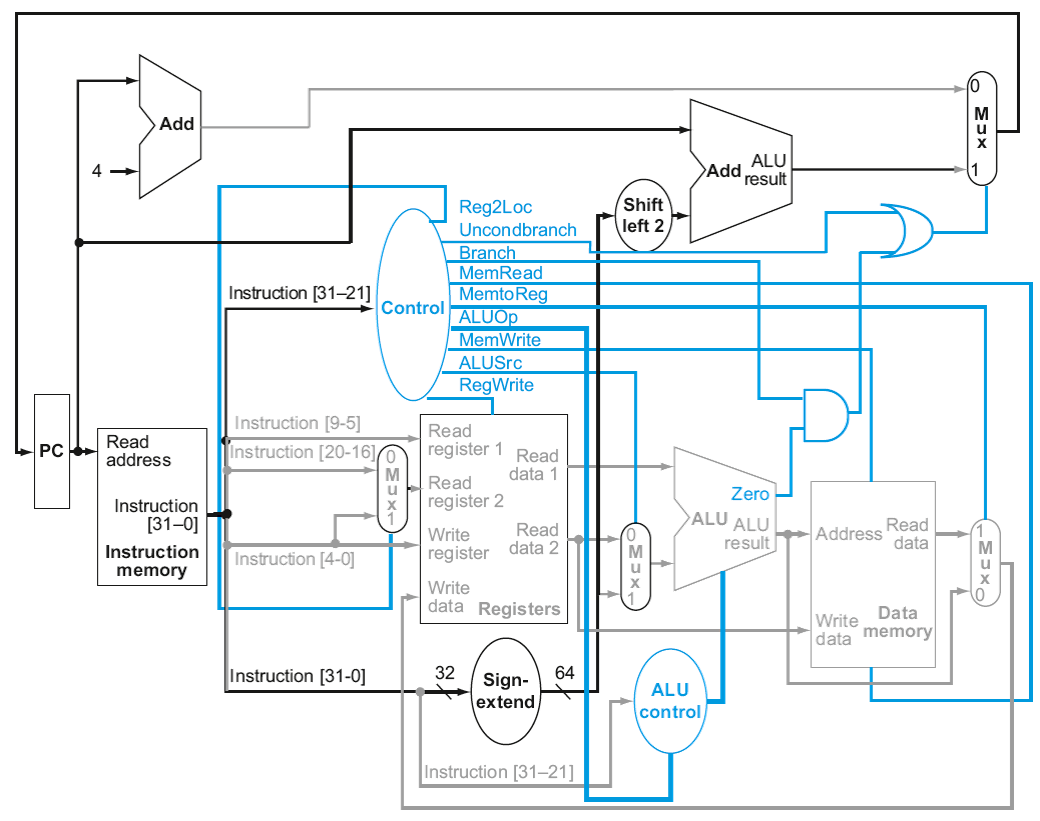
\includegraphics[width=\textwidth]{../images/non_pipelined_datapath.png}
\end{center}
\end{figure}

\section{Your Assignment}

You are to:
\begin{enumerate}
\item Update your Expected Results Table to include the iWriteBack stage.
\item Create the iWriteback stage consisting of one Mux.
\item Integrate all five stages into the file datapath.sv.
\item Run simulations to verify that your results match your Expected Results table.   
	\begin{enumerate}
	\item Your name and the lab number.
	\item A snip of the Simulation Results for both the datapath.sv test and division.sv.  Please show instructions in hex, opcodes and control signals in binary and everything else in signed decimal.  
	\item Copy and paste the entire log for both datapath.sv and division.sv from BEGIN TEST RESULTS to END TEST RESULTS into your file.  The results have gotten too long to use the snipping tool.	
\end{enumerate}
\item Upload Lab11\_lastname.pdf file to Canvas.
\item Zip up your ARM-Lab directory and submit it on Canvas as well.  Please make sure that you give me the ARM-Lab directory rather than the ARM-Project directory.  I do not want the project files in the ARM-Project directory.  Before you submit your zip file, extract the file and make sure that the top-level directory is called ARM-Lab and that the lower level directories like code, manual, etc are directly beneath ARM-Lab in the directory structure.  I will extract your zip file and run your code against my correct testbench to verify that your code and testbench work correctly, and it is critical that everyone's directory structure is consistent.
\end{enumerate} 
\chapter{Program Execution}

\section{Division}
To fully verify your LEGv8 processor, we are going to write a program that can divide two numbers, run that program and verify that we get the correct result.  The program that we will run is shown in the file division.c, shown below.  At the top of that file, I've listed some rules about the contents of the regData file and the ramData file.  I have included the assembly code for this simple division algorithm.  You will need to translate this assembly code into machine code.  We will use new testfiles for this program, so you need to create the following files in ARM-Lab/testfiles:
\begin{enumerate}
	\item instrData\_division.data - this file should contain the machine code for this division program 
	\item regData\_division.data - you must set all register values in regData\_division.data to 0 except for A22, which should be set to 24.  This value is the base address of the array A.  This is the only non-zero value allowed in regData.  
	\item ramData\_division -  this file should have all values set to 0 except for the values of A[0], A[1], A[2], and A[3].  Please set the dividend to 56 and the divisor to 8.  The quotient is initially set to 0.  A[3] is set to 1.  This is necessary because we do not have immediate instructions in our processor.
\end{enumerate}

To verify operation, you should create a final test bench (division.sv) that is the same as datapath.sv except that it allows pc\_src to be set by the iMemory module rather than keeping it hard-coded to 0 with pc\_src\_tmp.  These instructions are meant to run as a program and correct branch decisions are vital to its operation.  

The test bench verification is very simple.  It has only one test step, which verifies the value that is being stored by the final instruction.  Given that we are calculating 56/8, the result should be 7.  Rather than verifying hundreds of steps along the way (which we've already done), we will very simply check to see if the division works by checking the value of read\_data2 in the final instruction (STUR). Note that this single verify needs to occur at time=345ns.  

Feel free to also modify ramData\_division.data to use a different dividend and divisor and try out other calculations...but make sure that they are divisible.  57/8 (or anything like that) will not work properly, as it will never break out of the loop.

\Verilog{C code for doing simple division.}{code:division}{../code/division.c}
\Verilog{Assembly code for doing simple division.}{code:division_assembly}{../code/division_assembly.txt}


\section{Your Assignment}

You are to:
\begin{enumerate}
	\item Create and update division.sv.
	\item Run the simulation, analyze the results and verify that the divison works correctly.
	\item Rather than writing a lab report, please produce a landscape mode PDF file called Lab12\_lastname.pdf that includes (in this order):
	\begin{enumerate}
		\item Your name and the lab number.
		\item A snip of the Simulation Results for division.sv.  Please show instructions in hex, opcodes and control signals in binary and everything else in signed decimal.  
		\item Copy and paste the entire log for both datapath.sv and division.sv from BEGIN TEST RESULTS to END TEST RESULTS into your file.  The results have gotten too long to use the snipping tool.	
	\end{enumerate}
\item Upload Lab12\_lastname.pdf file to Canvas.
\item Zip up your ARM-Lab directory and submit it on Canvas as well.  Please make sure that you give me the ARM-Lab directory rather than the ARM-Project directory.  I do not want the project files in the ARM-Project directory.  Before you submit your zip file, extract the file and make sure that the top-level directory is called ARM-Lab and that the lower level directories like code, manual, etc are directly beneath ARM-Lab in the directory structure.  I will extract your zip file and run your code against my correct testbench to verify that your code and testbench work correctly, and it is critical that everyone's directory structure is consistent.
\end{enumerate} 

CONGRATULATIONS!  YOU'VE JUST BUILT A SIMPLE ARMv8 PROCESSOR!!!!
%\chapter{Full Datapath}


\section{Datapath}
Now that we have a working single-cycle datapath, we are going to break it apart and start pipelining it.  Make sure to keep a copy of your working single cycle datapath for reference.  To begin the pipelining process, we will first pipeline the iFetch and iDecode stages.

The advantage of pipelining includes the ability to reduce the clock cycle time by doing only one stage at a time.  We have been using a 10ns clock cycle.  Now that we are pipelining, let's start conservative and go down to a 4ns clock cycle.  Please keep it at 4ns for now to maintain consistency across the class.  

This will affect your timing and will require you to update your delays in your datapath.  Ask yourself why you made each delay.  Was it really meant to be relative to the clock cycle time, or was it meant to be a constant number. For instance, if you put in a CYCLE/10 to give a register time to update, do you really want that time to drop from 1ns to 0.4ns?  Has anything about the register update time changed?  The answer is no.  So you need to be strategic with your delays throughout these two stages.  You might also need to modify your delay functions.  The goal for today is to get a series of instructions to execute in pipeline form, where a new instruction is fetched while the previous instruction is being decoded.  You should verify this by examining the Read\_Register values, Read\_Data values, control signal values, etc.  The next step will be buffering nPC and the instruction, but we will focus on that next class.

To test this, use your set of instructions that corresponds to your Expected Results table.

\section{Your Assignment}

You are to:
\begin{enumerate}
\item Comment out Execute, Memory, and WriteBack stages from datapath.v.
\item Pipeline iFetch and iDecode stages and update delays.   
\item Test with your set of instructions from your Expected Results table.
\item Verify that stages are processing the correct instructions at the correct times.
\item There is no lab report today.
\end{enumerate} 
\chapter{Pipelining without Branching or Forwarding}


\section{Overview}
Now that we can pipeline stages and run them in parallel, we can add the register buffers between each stage and get a simple pipeline working.  This pipeline will not include any data forwarding or branch prediction.  We will handle data hazards by using assembly code with appropriately place nop commands to stall.  For now, we will avoid control hazards by not running any branch instructions.  We will focus on a series of load, arithmetic, and store instructions.

The first step is to create a spreadsheet using the template in this manual directory.  This spreadsheet should detail each input and output of the system.  It will then be filled in with data that needs to be buffered and passed to the next stage.  Please fill out the spreadsheet by doing the following:
\begin{enumerate}
	\item Add all of your inputs and outputs from each module, according to datapath.v.
	\item For each signal, identify the source and destination(s).
	\item For each signal, fill in stages that need the data to be buffered and passed along.  See mem\_to\_reg on template.
	\item For each signal (including the signals to pass along), label the signals with \_if, \_id, \_ie, \_im, or \_iw to indicate what stage that signal is coming from.
	\item Now consider any signals that need to be added due to pipelining, especially signals that go from right to left, such as the register write signals.  Add those to the spreadsheet.
	\item Think through the spreadsheet and determine if you have any holes in your design
\end{enumerate}  

Only after you have completed the spreadsheet as a group (work together on the spreadsheet) and have showed it to me, then you can move on to writing Verilog code.  You will want to update datapath.v to use the names from the spreadsheet.  This will include adding a lot of new signals.  Then you will want to update your modules to account for these new signals.  Try to change as few names as possible within the modules.  You want to use the stage-specific name in datapath.v rather than in the modules, to the extent possible.  Next, you will add procedural statements to assign inputs to register outputs (or in some cases, they will be registers that are internal to the module).  Compile and fix warnings.  Test files (instrData, regData, ramData) have been added to the repository.  Please use these files to test your code.  The assembly for those files is below:

\begin{enumerate}
\item LDUR X9, [X22 , \#0] ;     //load X9 from A[0], X22 = 80, A[0] = 56
\item LDUR X10, [X22 , \#8 ];    //load X10 from A[1], X22 = 80, A[1] = 8
\item LDUR X11, [X22 , \#16];    //load X11 from A[2], X22 = 80, A[2] = 35 
\item LDUR X12, [X22 , \#24];    //load X12 from A[3], X22 = 80, A[3] = 5
\item SUB X9, X9, X10 ; 
\item ADD X11, X11, X12 ; 
\item STUR X9,  [X22 , \#0]
\item STUR X11, [X22 , \#16]
\end{enumerate}
  


\section{Your Assignment}

You are to:
\begin{enumerate}
\item Finish the spreadsheet
\item Implement the spreadsheet in your datapath.v
\item Update your modules to buffer the appropriate values into registers
\item Use the test data files to test the pipeline and correct any issues
\item Submit a lab report using the PipelineLabWriteup format.
\end{enumerate} 
%\chapter{Pipelining with Branching}


\section{Overview}
Once your pipeline is working with the simple set of commands that I provided, it is time to add branching.  

We will put the following restrictions on our efforts to branch:
\begin{enumerate}
	\item Use Branch Not Taken method of prediction
	\item You should move the branch decision hardware to the Decode stage as mentioned in the lecture. 
	\item When a branch is taken, you must zero the control lines and set PCWrite and IF/IDWrite to 0.  You will need to add PCWrite and IF/IDWrite.  Branch hazards must be detected by a new module, the Hazard Detection Unit.
	\item Instructions used for this should be the division problem instructions.  You need to insert nops (all zeros) in the instruction file where necessary.  The only reason to add nops in the instruction file is a data hazard
\end{enumerate}  

\section{Your Assignment}

You are to:
\begin{enumerate}
\item Implement Branch Not Taken Prediction
\item Create an instruction file as described above, based on the division problem instruction file
\item Update your modules to detect and respond to branch hazards
\item Use the instruction to test the pipeline and correct any issues
\item Submit picture(s) of your simulation results.  Also submit a zip file of your repository.
\end{enumerate} 

\end{document} 